\section{Datenerfassung}\label{sec:Datenerfassung}
Die Herausforderung beim Auslesen der Daten liegt darin, die plattformspezifischen Informationen in einem allgemeinen Datenmodell zu konsolidieren. Hierbei stammen die Daten aus verschiedenen Schnittstellen. Die Architektur muss in der Lage sein, sämtliche verfügbaren Sensordaten plattformunabhängig auszulesen, darunter beispielsweise Temperaturen und CPU-Auslastung. Zusätzlich sollte sie die Integration weiterer plattformspezifischer Hardwarekonfigurationen und Schnittstellen ermöglichen, ohne eine grundlegende Neustrukturierung des bestehenden Codes zu erfordern.\\
Das Speichern der ausgelesenen Messdaten soll in einem einheitlichen Format erfolgen, das unabhängig von der Hardwarekonfiguration der Zielplatform ist. Zudem ist eine klare und sinnhafte Struktur der Datenbank wichtig, da diese Performant und Skalierbar sein muss.   

\subsection{Entwurf einer Architektur zum Auslesen der Systemhardware}\label{sec:AuslesenHardware}
 
Die Objekte und Klassen, die für das Auslesen der Systemhardware verwendet werden, sind im Verzeichnis \textit{HM.HWServices} abgelegt. Dieses Verzeichnis enthält alles, was benötigt wird, um die Hardware der Zielplatformen auszulesen.\\
Das UML Diagramm in Abbildung \ref{fig:HWServicesUML} veranschaulicht den Aufbau von \textit{HM.HWServices}. 
\begin{center}
    \begin{figure}[h!]
        \centering
        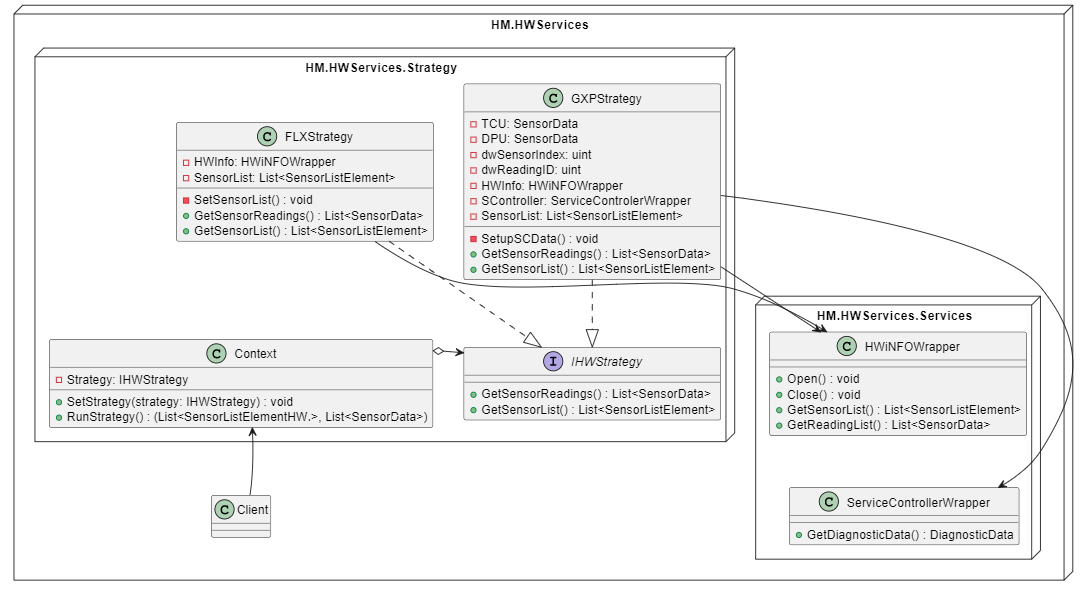
\includegraphics[width=1\textwidth]{UMLDatenerfassung.png}
        \caption{Architektur der HM.HWServices für das Auslesen der Hardware}
        \label{fig:HWServicesUML}
    \end{figure}
\end{center}
\vspace{-1.8cm}
Die Architektur der \textit{HM.HWServices} wird nach dem, in Abschnitt \ref{sec:StrategyPattern} beschriebnen Strategie Muster ausgelegt.
Die Komponenten des Strategie Musters sind im Verzeichnis \textit{HM.HWServices.Strategy} organisiert.\\
Durch den \textit{Context} kann die gewünschte Strategie ausgewählt und aufgerufen werden. Die Client-Anwendung interagiert dabei ausschließlich mit dem \textit{Context}, der wiederum die gewünschten Funktionen der ausgewählten Strategieklasse aufruft.\\  
Da sich das Auswerten von VisuNet FLX und GXP voneinander unterscheidet, soll für jede Platform eine eigene Strategieklasse verantwortlich sein. Jede dieser Strategieklasse wird hierbei von dem \textit{IHWStrategy} Interface abgeleitet. Dieses definiert die Struktur der Klassen, sodas die Funktion der ausgewählten Klasse im \textit{Context} ausgeführt werden kann, ohne die spezifische Strategieklasse genau zu kennen. Anschließend kann beim Start des Programms entschieden werden, welche dieser Strategien angewendet werden soll.\\
Muss das Programm in Zukunft um eine neue Hardwarekonfiguration einer Platform erweitert werden, kann dies über das hinzufügen einer weiteren Strategieklasse realisiert werden.\\
Zum Auslesen der Sensordaten stehen zunächst zwei Schnittstellen zurverfügung. Zum einen liefert über die in Abschnitt \ref{sec:HWiNFO} beschriebene Shared Memory Funktion der HWiNFO Software Messwerte aller an das Mainboard angeschlossenen Sensoren. Die VisuNet FLX Platform bedarf keiner weiteren Schnittstellen zum lesen von Sensordaten.\\
Um die Temperatursensoren in \ac{dpu} und \ac{tcu} der VisuNet GXP Plattform aus zu lesen, wird eine Weitere Bibliothek verwerwendet, welche die Komunikation mit dem in der Platform verbauten Servicecontroller ermöglicht.\\
Für beide Schnittstellen wurde eine Wrapperklasse (Siehe Abschnitt \ref{sec:AdapterPattern}) konzipiert, welche die wesentlichen Funktionen in einer übersichtlichen Klasse bereitstellen und die Datenstruktur der Schnittstelle adaptieren. Die Wrapperklassen werden im Verzeichnis \textit{HM.HWServices.Wrapper} organisiert. Die Wrapperklassen sind in Abbildung \ref{fig:HWServicesUML} zu sehen.
\subsubsection*{Adaption der Schnittstelle}
Beim Auslesen der Sensorik über die \textit{HWiNFOWrapper} Klasse, können zwei Listen ausgelesen werden. Zum einen werden alle verfügbaren Sensoren der Platform in einer Liste von \textit{SensorListElement} abgelegt. Zum anderen wird eine Liste des Typen \textit{SensorData} erzeugt. In dieser ist jeder Sensor mit dem aktuellen Messwertwert hinterlegt. Die Datentypen hierzu sind in Abbildung \ref{fig:DatastructuresUML} abgebildet.      
\begin{center}
    \begin{figure}[h!]
        \centering
        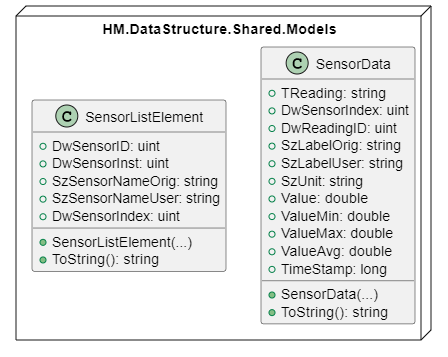
\includegraphics[width=0.45\textwidth]{UMLDatastructureHWI.png}
        \caption{Datenstruktur zum zwischenspeichern der Sensordaten}
        \label{fig:DatastructuresUML}
    \end{figure}
\end{center}
\vspace{-1.8cm}

\subsubsection*{Strategie Konzept}
Ziel der Strategieklassen ist wie zuvor bereits erwähnt die Kapselung der Algorithmen zum Auslesen der Zielplatformen. Eine Strategie soll daher folgende daten zurück liefern: Zum einen soll eine Aufzählung aller Sensoren im System erstellt werden, und in einer Liste von \textit{SensorListElement} hinterlegt werden. (Siehe Tabelle \ref{fig:SensorList}) 
\vspace{-0.5cm}
\begin{center}
    \begin{table}[h!]
        \centering
        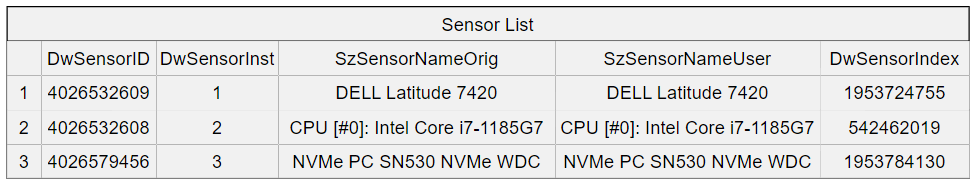
\includegraphics[width=0.7\textwidth]{SensorList.png}
        \caption{Beispiel einer Liste bestehend aus \textit{SensorListElement}}
        \label{fig:SensorList}
    \end{table}
\end{center}
\vspace{-1.8cm}
Zum anderen soll ein aktueller Auszug der Sensorwerte erstellt werden können. Hierzu sollen die Werte der einzelnen Sensoren in einer Liste von \textit{SensorData} gespeichert werden. (Siehe Tabelle \ref{fig:SensorReadings})
\vspace{-0.5cm}
\begin{center}
    \begin{table}[h!]
        \centering
        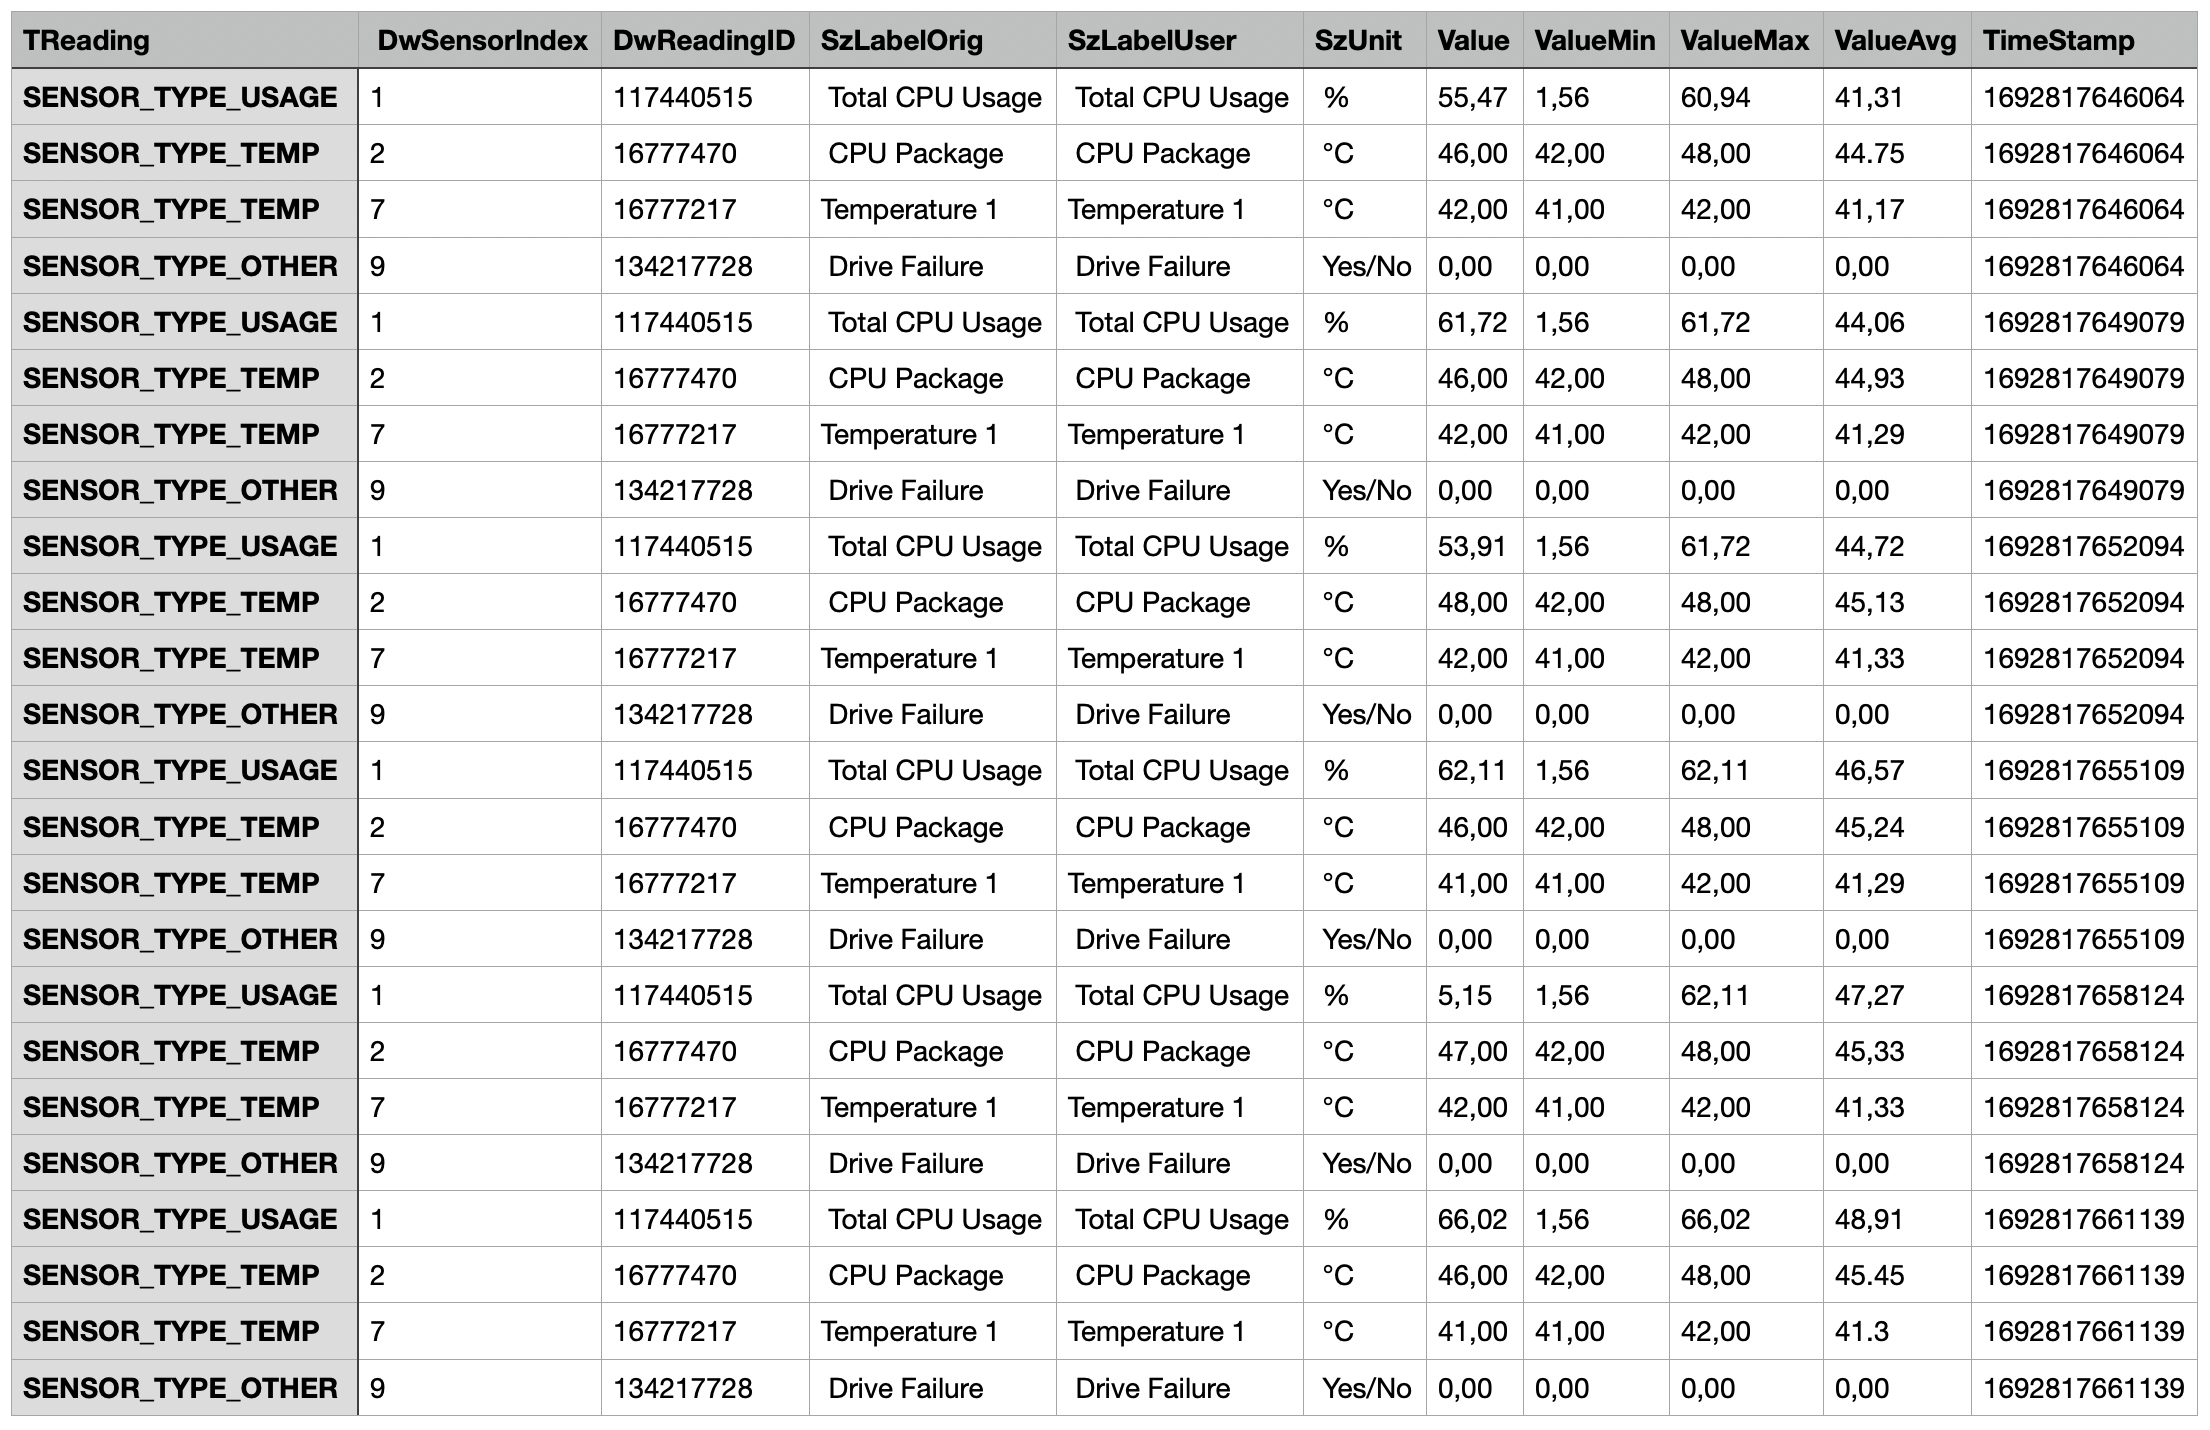
\includegraphics[width=0.81\textwidth]{SensorReadings.png}
        \caption{Beispiel einer Liste bestehend aus \textit{SensorData}}
        \label{fig:SensorReadings}
    \end{table}
\end{center}
\vspace{-1.8cm}
Da die \textit{HWiNFOWrapper} Schnittstelle alle verfügbraren Sensoren der VisuNet FLX Platform abdekt, ist die Strategie zum Auslesen dieser Platform recht Simpel. Dabei soll über einen Funktionsaufruf eine Liste mit den Aktuellen Messwerten der Sensoren erstellt und zurückgegeben werden.\\
Der \textit{ServiceControllerWrapper} liefert, neben dem werten des \textit{HWiNFOWrapper}, \ac{dpu} und \ac{tcu} Temperaturen der VisuNet GXP Platform. Die Datensätze der beiden Schnittstellen müssen daher in der \textit{GXPStrategy} kombiniert werden, sodas wie auch bei der \textit{FLXStrategy} jeweils eine Liste der Sensoren und eine Liste mit den Messwerten erstellt wird (Siehe Tabelle \ref{fig:SensorList} und \ref{fig:SensorReadings}).\\
Mithilfe der Strategieklassen kann somit für jegliche Hardwarekonfiguration einer Platform, eine gezielte Strategie erstellt werden, welche lediglich zwei Listen zurückliefert. Dabei ist der Anwendung selbst egal welche und wieviel Schnittstellen verwendet werden.

\subsection{Entwurf eines Datenbankmodells zum Speichern der Messwerte}
Im vorherigen Abschnitt \ref{sec:AuslesenHardware} wurde eine Architektur zum Auslesen der plattformunabhängigen Sensoren beschrieben. Resultierend daraus steht dem Programm eine Schnittstelle bereit, welche eine Reihe von Messdaten zur verfügung stellt. Ziel des Datenbankmodells ist es die bereitgestellten Messdaten in einem strukturierten und übersichtlichen Format ab zu speichern.\\

\subsubsection*{Zuordnung der Datensätze}
Aus Tabelle \ref{fig:SensorReadings} geht hervor das die Datensätze der SensorData Tabelle grundsätzlich in 3 kattegorien unterteilt werden können. Anhand der Spalte \textit{SzUnit} können die Daten in drei Kattegorien Temperatur (°C), Auslastung (\%) und Events (Yes/No) unterteilt werden. Bei weiterer Betrachtung der Datensätze wird zudem ersichtlich, das die Spalten \textit{TReading}, \textit{DwSensorIndex}, \textit{DwReadingID}, \textit{SzLabelOrig}, \textit{SzLabelUser} und \textit{SzUnit} bei jedem Sensor wiederholen.\\
Einhergehend aus diesen Beoabahtung wurde die in Abbildung \ref{fig:DBModell} abgebildete Struktur der Datenbank erstellt. 
\begin{center}
    \begin{figure}[h!]
        \centering
        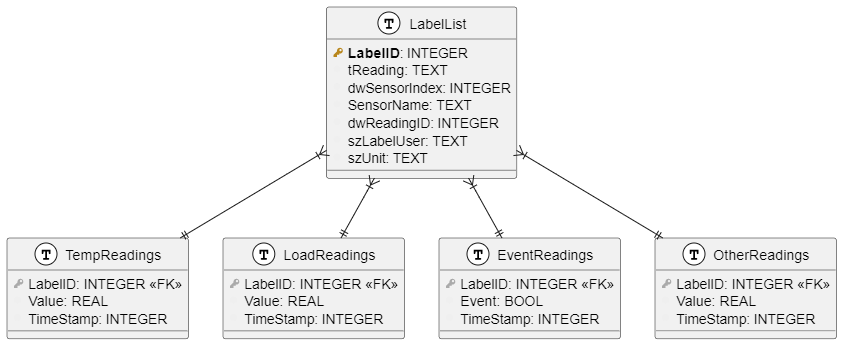
\includegraphics[width=1\textwidth]{DBModell.png}
        \caption{Datenbankmodell des Hardware-Health-Monitorings}
        \label{fig:DBModell}
    \end{figure}
\end{center}
\vspace{-1.8cm}
Die Datensätze der Tabellen \ref{fig:SensorList} und \ref{fig:SensorReadings} werden in 5 Datenbank Tabellen unterteilt. Dabei werden die Felder \textit{TReading}, \textit{DwSensorIndex}, \textit{DwReadingID}, \textit{SzLabel} und \textit{SzUnit} in die Tabelle \textit{LabelList} ausgelagert. Hinzu kommt das Feld \textit{SensorName}, welches aus Tabelle \ref{fig:SensorList} stammt. Über das Feld \textit{LabelID}, welches als Primär Schlüssel konfiguriert wird. Über diesen Schlüssel können nun die eigentlichen Messwerte, den Sensoren Zugeordnet werden. Die Messwerte werden dabei sortiert nach \textit{SzUnit} in vier Tabellen geschrieben. \textit{TempTabel} für Temperaturen in  °C, \textit{LoadReadings} für Auslastung in \%, \textit{EventTabel} für Events in 1/0 und \textit{OtherReadings} für alle andere Einheiten. Jede der vier Tabellen verfügt über ein Feld \textit{Value}, \textit{TimeStamp} und einer zugehörigen Schlüssel \textit{LabelID}.\\
Möchte man eine Reihe von messwerten eines Spezifischen Sensors erhalten, muss man zunächst den Primär Schlüssel des Sensors aus der \textit{LabelList} Tabelle ermitteln. Anschließend kann man die werte der entsprechenden Tabelle erhalten.

\subsubsection*{Erweiterung der Datenbank}
Zusätzlich zu den Ausgelesenen Messwerten, müssen auch die Ergebnisse der System Bewertung in der Datenbank abgelegt werden. 
Hierzu werden zunächst die Tabelle \textit{SystemStatus} und \textit{SystemMTBF} erstellt. Diese sind Identisch und unterscheiden sich lediglich in der Bedeutnug ihrer Werte. Der ermittelte Systemzustand wird in die Feldern \textit{Status}, \textit{Score} und \textit{Value} geschrieben. Die Felder \textit{TimeStampStart} und \textit{TimeStampEnd} grenzen das Interval, in welchem der Systemzustand ermittelt wurde ein. Des weiteren werden die Tabellen \textit{HistorySystemStatus} und \textit{SystemReliability} erzeugt. Diese Speichern die Historischen Werte des Systems, so wie dessen Verlässlichkeit ab. (Siehe Abbildung \ref{fig:DBModellErweitert})   
\begin{center}
    \begin{figure}[h!]
        \centering
        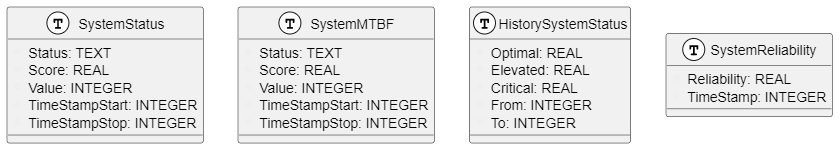
\includegraphics[width=1\textwidth]{DBErweitert.png}
        \caption{Datenbankmodellerweiterung des Hardware-Health-Monitorings}
        \label{fig:DBModellErweitert}
    \end{figure}
\end{center}
\vspace{-1.8cm}

\subsubsection*{Aufbau der Schnittstelle}
- komplizierte Syntax -> bedarf einer Abstraktion\\
- Datenbank wird über seperate Wrapperklasse ausgelesen und beschrieben. Hierzu Funktionen welche die datenbank beschreiben und auch wieder auslesen können. \\
- einführung der \textit{ValueReading}. Wird verwendet um eine Reihe von sensordaten abzu speichern. \\
- Funktionen zum auslesen bestimmter sensordaten, bezogen auf einen bestimmts intervall\\




















